\subsection{Inducción magnética}

Como este documento es un resumen de la materia Física II y no un libro de física, no voy a entrar en detalles de la inducción magnética, ya que este tema solo se presenta conceptualmente en la materia. Para no dejar de lado el tema, voy a presentar la ecuación que describe el fenómeno de inducción magnética de forma general.

\subsubsection{Ley de Faraday}

La ley de Faraday describe cómo un campo magnético variable en el tiempo puede generar una fuerza electromotriz (fem), es decir, una diferencia de potencial capaz de inducir una corriente eléctrica en un circuito conductor. Este fenómeno se conoce como inducción electromagnética.

La ley de Faraday establece que la fuerza electromotriz inducida en un circuito cerrado es igual (en magnitud) a la rapidez con que varía el flujo magnético a través de la superficie delimitada por ese circuito.

Matemáticamente, en su forma integral:
\[
  \mathcal{E} = -\frac{d\Phi_B}{dt}
\]
donde:
\begin{itemize}
  \item \(\mathcal{E}\) es la fem inducida (en voltios),
  \item \(\Phi_B\) es el flujo magnético a través de una superficie $S$, definido como: \(\Phi_B = \int_S \vec{B} \cdot d\vec{A}\),
  \item \(\vec{B}\) es el campo magnético (en teslas),
  \item \(d\vec{A}\) es el vector diferencial de área orientada perpendicularmente a la superficie,
\end{itemize}

El signo negativo proviene de la ley de Lenz que se describe con más detalle en la siguiente sección (\ref{sec:ley_de_lenz}), que indica que la corriente inducida genera un campo magnético que se opone al cambio del flujo que la produce (principio de conservación de la energía).

Lo que nos dice la ley de Faraday es que si un campo magnético cambia con el tiempo (ya sea porque aumenta, disminuye o varía su orientación), y hay un conductor cerrado (como una espira), entonces se induce una corriente eléctrica en dicho conductor.
También puede inducirse corriente si el conductor se mueve dentro de un campo magnético constante, cambiando así el flujo que lo atraviesa.

\subsubsection{Ley de Lenz}
\label{sec:ley_de_lenz}

La ley de Lenz describe la dirección de la corriente eléctrica inducida por un campo magnético variable, y es una consecuencia del principio de conservación de la energía.

\begin{figure}[ht]
  \centering
  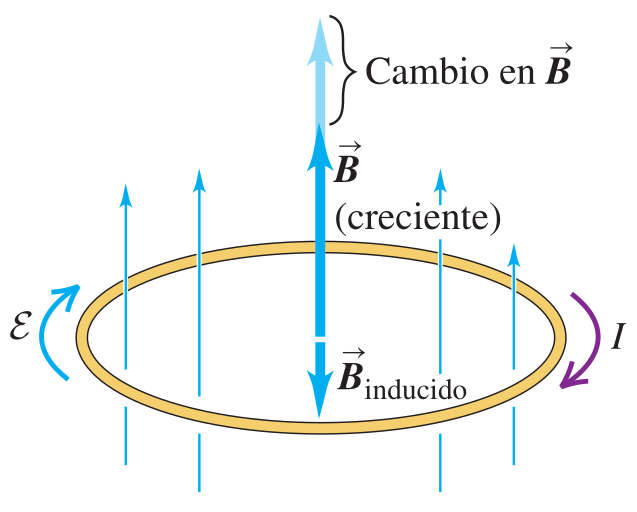
\includegraphics[width=0.4\textwidth]{electromagnetic_induction.png}
  \caption{La variación del campo magnético crea un campo magnético que se opone al cambio del flujo que la produce.}
  \label{fig:electromagnetic_induction}
\end{figure}

Esta ley puede enunciar así:

\begin{tcolorbox}[myconclusion]
  La corriente inducida por un cambio en el flujo magnético tiene una dirección tal que el campo magnético que genera se opone al cambio del flujo que la produce.
\end{tcolorbox}

Este enunciado es fundamental para determinar el signo negativo que aparece en la ley de Faraday:

$$
\mathcal{E} = -\frac{d\Phi_B}{dt}
$$

El signo negativo expresa matemáticamente lo que la ley de Lenz establece cualitativamente: la inducción electromagnética se resiste al cambio que la origina.

Desde el punto de vista de la mecánica clásica:
\begin{itemize}
  \item Si el flujo magnético a través de una espira aumenta, la corriente inducida genera un campo magnético opuesto, intentando reducir ese aumento.
  \item Si el flujo magnético a través de una espira disminuye, la corriente inducida genera un campo magnético opuesto, intentando restaurarlo.
\end{itemize}

Este comportamiento garantiza que no se cree energía de la nada, respetando la conservación de la energía.

Un ejemplo sencillo: si acercamos un imán a una espira de alambre, se induce una corriente. Esa corriente genera un campo magnético que se opone al movimiento del imán. Es decir, la espira actúa como un ``freno magnético'' que resiste el alejamiento o acercamiento del imán como se muestra en la figura \ref{fig:electromagnetic_induction}.

La ley de Lenz garantiza que para inducir una corriente, se debe realizar un trabajo mecánico. Por ejemplo, al mover un imán hacia una bobina, se debe vencer la fuerza inducida que se opone al movimiento. Esa energía mecánica se transforma en energía eléctrica.